\chapter{Analisis}
\section{Arsitektur Perangkat Lunak}
Untuk membangun sebuah perangkat lunak yang dapat memprediksi kemacetan diperlukan sebuah arsitektur yang mencakup pengambilan data, pra proses, dan pemprosesan data hingga menghasilkan output.
\begin{figure}
\centering
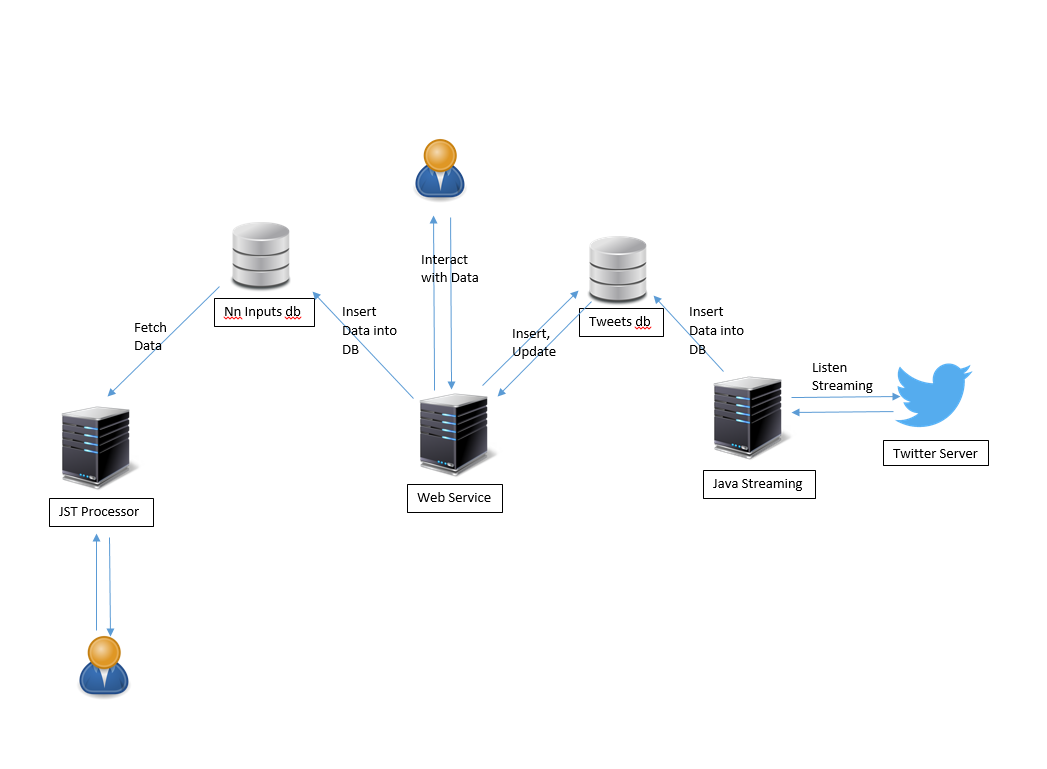
\includegraphics[width=\linewidth]{Gambar/mine/sistem}
\caption[Arsitektur Perangkat Lunak]{Arsitektur Perangkat Lunak} 
\label{fig:arsitekturpl}
\end{figure}
\section{Menarik Input}
\section{Rancangan Basis Data}